\documentclass[tikz,border=3pt]{standalone}
\usepackage[T1]{fontenc}
\usepackage{lmodern}
\usetikzlibrary{arrows.meta,positioning,fit,backgrounds}
\definecolor{ink}{RGB}{24,39,53}
\definecolor{blue}{RGB}{36,82,126}
\definecolor{pale}{RGB}{239,245,250}
\definecolor{teal}{RGB}{34,108,104}
\definecolor{warm}{RGB}{153,88,42}
\begin{document}

% Cells share one height and start at the top; no hyphenation inside the narrow cells.
\newcommand{\cell}[2]{\parbox[t][2.2cm][t]{3.6cm}{\raggedright\hyphenpenalty=10000\exhyphenpenalty=10000
 \textbf{#1}\\[4pt]#2}}
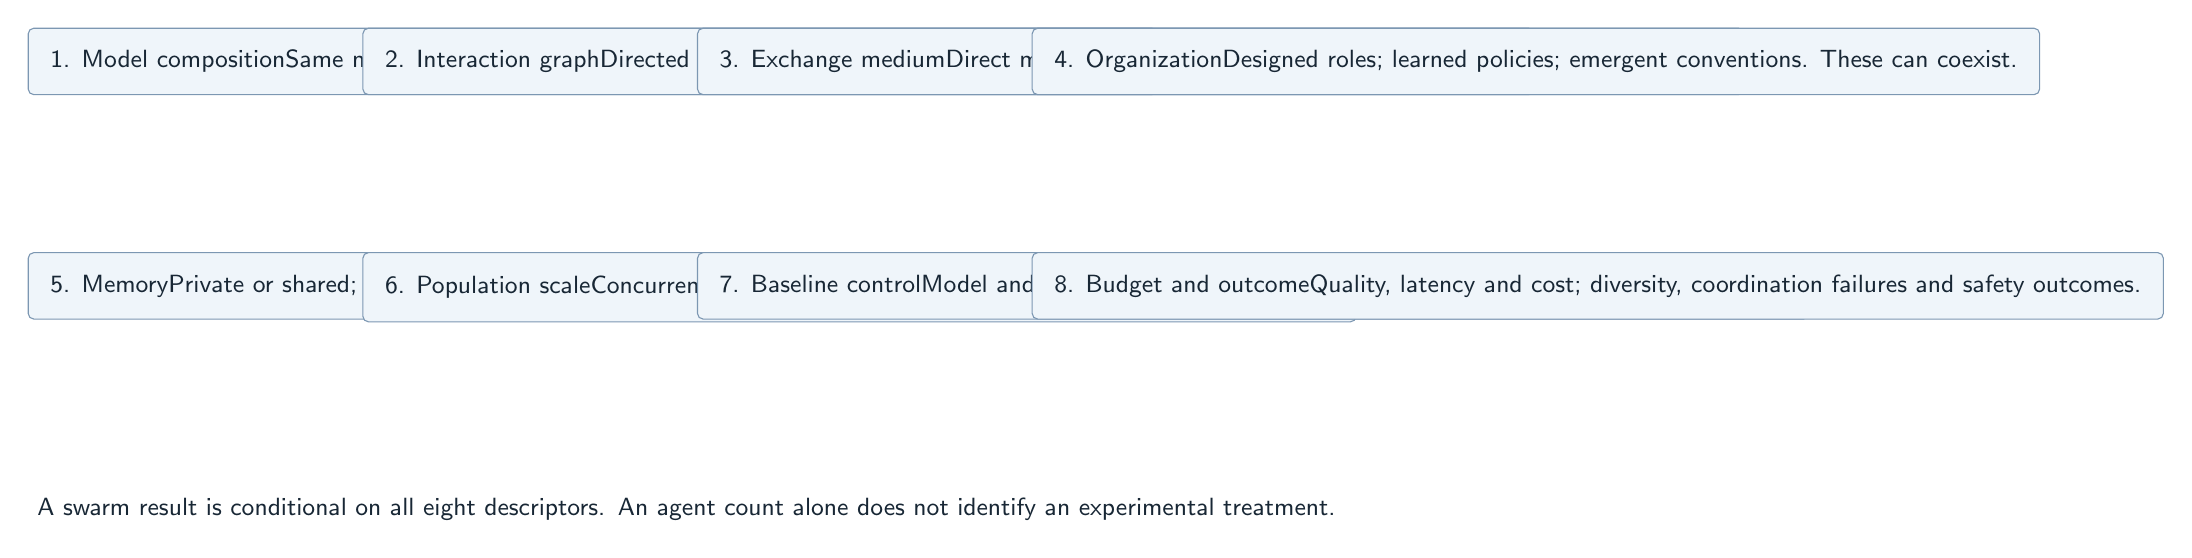
\begin{tikzpicture}[font=\sffamily\small, text=ink,
  box/.style={draw=blue!60,rounded corners=2pt,fill=pale,inner sep=8pt,anchor=north west}]
\node[box] (a) at (0,0) {\cell{1. Model composition}{Same model or mixed models; role prompts; competence and error correlations.}};
\node[box] (b) at (4.25,0) {\cell{2. Interaction graph}{Directed or undirected; dense or sparse; fixed or dynamic; allowed and realized edges.}};
\node[box] (c) at (8.5,0) {\cell{3. Exchange medium}{Direct messages, shared files, repositories, tools, or an external platform.}};
\node[box] (d) at (12.75,0) {\cell{4. Organization}{Designed roles; learned policies; emergent conventions. These can coexist.}};
\node[box] (e) at (0,-2.85) {\cell{5. Memory}{Private or shared; lifetime; retrieval and updates; provenance and access control.}};
\node[box] (f) at (4.25,-2.85) {\cell{6. Population scale}{Concurrent $N_{\mathrm{conc}}(t)$; cumulative $N_{\mathrm{cum}}(T)$; configured capacity $N_{\mathrm{cap}}$.}};
\node[box] (g) at (8.5,-2.85) {\cell{7. Baseline control}{Model and tasks; tools and context; tokens, compute, dollars, or wall-clock time.}};
\node[box] (h) at (12.75,-2.85) {\cell{8. Budget and outcome}{Quality, latency and cost; diversity, coordination failures and safety outcomes.}};
\node[anchor=north west,align=left,font=\sffamily\small,text width=16.7cm] at (0,-5.85)
 {A swarm result is conditional on all eight descriptors. An agent count alone does not identify an experimental treatment.};
\end{tikzpicture}
\end{document}
